\documentclass{article}
\usepackage{graphicx} % Required for inserting images
\usepackage[T2A]{fontenc}
\usepackage{titlesec}
%\usepackage{verbatim}
\usepackage[left=25mm, right=15mm, top=20mm, bottom=20mm, footskip=10mm]{geometry}
\usepackage{amsmath}
\usepackage{epigraph}
\usepackage{tikz}
\usepackage{latexsym}
%\usepackage{listings}
\frenchspacing 
\newcommand{\path}{\rightsquigarrow}
\titleformat{\section}[hang]{\normalsize\bfseries}{\thesection~}{0pt}{}
\titlespacing{\section}{\parindent}{\baselineskip}{\baselineskip}

\titleformat{\subsection}[hang]{\normalsize}{\thesubsection~}{0pt}{}
\titlespacing{\subsection}{\parindent}{0pt}{0pt}
\parindent=1.25cm 

\title{Тема 5. Компоненты сильной связности, конденсация графа }
\date{}

\begin{document}

\maketitle

\epigraph{Автор конспекта: Родион Лыков}


\section{Определения}

\begin{enumerate}
    \item \textbf{Полустепень захода} вершины $x$ орграфа называется количество ребер, входящих 
    в вершину $x$.  
    \item \textbf{Полустепень исхода} вершины $x$ орграфа называется количество ребер, выходящих 
    из вершины $x$.
    \item \textbf{Истоком} называется такая вершина $x$, в которую не входят ребра. Иными словами, полустепень захода равна нулю: $deg^{+}(x)=0$.
    \item \textbf{Стоком} называется такая вершина $x$, из которой не выходят ребра. Иными словами, полустепень исхода равна нулю: $deg^{-}(x)=0$.
    \item \textbf{Изолированной} называется такая вершина $x$, что обе степени захода и исхода равны нулю. 
    \item \textbf{Компонентной слабой связности графа} называется такое максимальное подмножество вершин, что если бы ребра не имели ориентации, то из любой вершины можно было бы дойти до любой другой. 
    \item \textbf{Компонентной сильной связности графа} называется такое максимальное подмножество вершин, что из любой вершины можно дойти до любой другой. 
    \item Граф называют \textbf{слабо связным}, если он состоит из одной компоненты слабой связности.
    \item Граф называют \textbf{сильно связным}, если он состоит из одной компоненты сильной связности.
\end{enumerate}

Приведем примеры:
\begin{enumerate}
    \item Пример графа, с тремя компонентами слабой связности:
    \begin{center}
        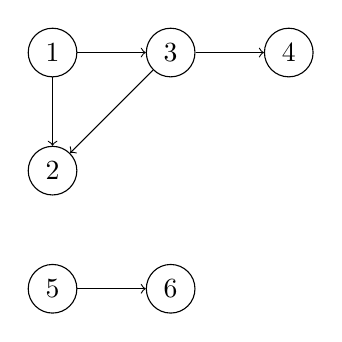
\begin{tikzpicture}[main/.style = {draw, circle},node distance={15mm}] 
        \node[main] (1) []{$1$}; 
        \node[main] (2) [below of=1] {$2$}; 
        \node[main] (3) [right of=1] {$3$}; 
        \node[main] (4) [right of=3] {$4$};
        \node[main] (5) [below of=2] {$5$};
        \node[main] (6) [right of=5] {$6$};
        \draw[->] (1) -> (2);
        \draw[->] (3) -> (2);
        \draw[->] (1) -> (3);
        \draw[->] (3) -> (4);
        \draw[->] (5) -> (6);
        \end{tikzpicture} 
    \end{center}
    В этом графе есть компоненты: $[1,2,3,4]$ и $[5,6]$.
    \item Пример компоненты сильной связности:
    \begin{center}
        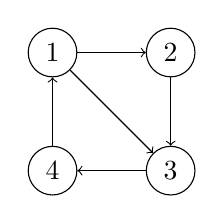
\begin{tikzpicture}[main/.style = {draw, circle},node distance={15mm}] 
        \node[main] (1) []{$1$}; 
        \node[main] (2) [right of=1] {$2$}; 
        \node[main] (3) [below of=2] {$3$}; 
        \node[main] (4) [left of=3] {$4$};
        \draw[->] (1) -> (2);
        \draw[->] (2) -> (3);
        \draw[->] (3) -> (4);
        \draw[->] (4) -> (1);
        \draw[->] (1) -> (3);
        \end{tikzpicture} 
    \end{center}
\end{enumerate}

\section{Тип графа: DAG}

Очень часто в задачах вы работаете с таким типом графов, как DAG (Directed acyclic graph) или же Ориентированный граф без циклов. Вот так, например, он выглядит: 

\begin{center}
        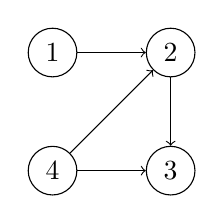
\begin{tikzpicture}[main/.style = {draw, circle},node distance={15mm}] 
        \node[main] (1) []{$1$}; 
        \node[main] (2) [right of=1] {$2$}; 
        \node[main] (3) [below of=2] {$3$}; 
        \node[main] (4) [left of=3] {$4$};
        \draw[->] (1) -> (2);
        \draw[->] (2) -> (3);
        \draw[->] (4) -> (3);
        \draw[->] (4) -> (2);
        \end{tikzpicture} 
    \end{center}
Как видите, цикла в таком графе нет. Давайте рассмотрим несколько заявлений:
\begin{enumerate}
    \item В DAG'e всегда есть исток и сток. Докажем это очень просто: 
    рассмотрим любую вершину $x$ и выберем из нее случайное ребро, будем 
    так делать дальше, если мы пришли в вершину, из которой ничего не выходит, то мы пришли в сток. Но что если мы никогда не придем в такую вершину? Значит, каждый раз мы находим новое ребро, но так как ребер ограниченное количество, то когда-то мы перешли по ребру, по которому мы уже ходили, а значит попали в цикл. Но в графе циклов нет. Исток доказывается аналоично, нужно просто развернуть ребра графа.
    \item В DAG'e на $n$ вершинах $n$ компонент сильной связности
\end{enumerate}
Итак. Давайте решим следующую задачу на DAG'e: найдите все такие вершины, что из них можно дойти до всех других вершин. Сразу заметим тот факт, что в исток никогда не получится дойти, значит стартовая вершина должна быть истоком. Но если истоков несколько, то из одного истока мы в другой не попадем. Значит, в графе должен быть один исток и он же будет ответом. Попробуйте доказать, что если в графе один исток, то из него всегда можно дойти до других вершин.
Итак, напишем код:

\begin{verbatim}
#include <bits/stdc++.h>
using namespace std;
int n,m;
vector<vector<int>>color;
vector<vector<int>>e;

int main() {
    ios::sync_with_stdio(0);
    cin.tie(0);
    cout.tie(0);
    cin >> n >> m;
    e = vector<vector<int>>(n+1);
    for(int i = 1; i <= m; i++) {
        int x,y;
        cin >> x >> y; // считываем ребра
        e[x].push_back(y);
    }
    vector<int>in(n+1),out(n+1); // будем считать степени вершин графа, вход и выход
    for(int x = 1; x <= n; x++) {
        for(auto& y : e[x]) {
            // ребро x->y, тогда:
            out[x]++;
            in[y]++;
        }
    }
    int ans = -1;
    int cnt = 0; // считаем количество истоков
    for(int x = 1; x <= n; x++) {
        if(in[x] == 0) {
            ans = x;
            cnt++;
        }
    }
    if(cnt == 1) cout << ans << '\n'; // если исток один, то выводим его
    else cout << "No answer" << '\n';
}
\end{verbatim}

Итак, задача решена. Теперь решим следующую задачу: нам дан орграф, найдите все такие вершины, что из них можно пройти до всех других. Заметьте, тут уже могут быть циклы.

    \begin{center}
        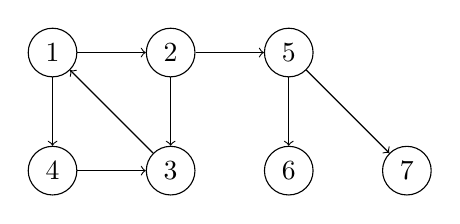
\begin{tikzpicture}[main/.style = {draw, circle},node distance={15mm}] 
        \node[main] (1) []{$1$}; 
        \node[main] (2) [right of=1] {$2$}; 
        \node[main] (3) [below of=2] {$3$}; 
        \node[main] (4) [left of=3] {$4$};
        \node[main] (5) [right of=2] {$5$};
        \node[main] (6) [below of=5] {$6$};
        \node[main] (7) [right of=6] {$7$};
        \draw[->] (1) -> (2);
        \draw[->] (1) -> (4);
        \draw[->] (4) -> (3);
        \draw[->] (3) -> (1);
        \draw[->] (2) -> (3);
        \draw[->] (2) -> (5);
        \draw[->] (5) -> (6);
        \draw[->] (5) -> (7);
        \end{tikzpicture} 
    \end{center}
В этом графе ответом являются вершины $[1,2,3,4]$. 
Для того, чтобы решить такую задачу, научимся делать конденсацию графа. 
Конденсация графа сжимает компоненты сильной связности в одну вершину. 
В этом графе есть компоненты сильной связности $[1,2,3,4], [5], [6], [7]$. 
Так как в компоненте сильной связности вы \textbf{можете дойти из любой вершины до любой другой}, то и по ребру $(2,5)$ вы сможете всегда перейти. Таким образом, не важно, в какой вершине компоненты сильной связности мы находимся. После конденсации граф будет выглядеть вот так:
\begin{center}
        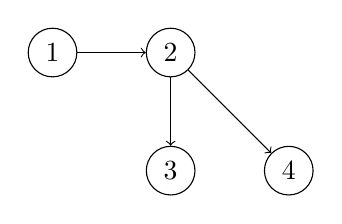
\begin{tikzpicture}[main/.style = {draw, circle},node distance={15mm}] 
        \node[main] (1) []{$1$}; 
        \node[main] (2) [right of=1] {$2$}; 
        \node[main] (3) [below of=2] {$3$}; 
        \node[main] (4) [right of=3] {$4$};
        \draw[->] (1) -> (2);
        \draw[->] (2) -> (3);
        \draw[->] (2) -> (4);
        \end{tikzpicture} 
    \end{center}
Здесь в вершину $1$ залезла вся компонента $[1,2,3,4]$. 

\textbf{После конденсации в графе не будет циклов}. Это так, иначе мы бы могли сделать еще одну компоненту сильной связности, ведь в цикле можно дойти из любой вершины до любой другой. 
\textbf{Мы перешли к задаче на DAG'e, когда нет циклов}. Чтобы решить задачу на DAG'e нужно просто \textbf{Посчитать степени вершин и найти исток}. Причем исток должен быть единственным, смотрите задачу выше. 

Итак, конденсацию можно написать вот так: сначала запустим алгоритм поиска топологической сортировки, он нам, конечно, сам топсорт не найдет, ведь в графе могут быть циклы, но нам важно, что первая вершина в порядке <<топсорта>> будет в компоненте-истока. Теперь запустим из нее dfs и дойдем до всех вершин, до которых можем: но ведь мы можем уйти за компоненту: посмотрите на граф еще раз, если мы запустимся из вершины $4$, то мы вообще посетим все вершины графа. 
\begin{center}
        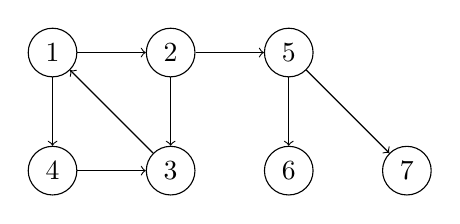
\begin{tikzpicture}[main/.style = {draw, circle},node distance={15mm}] 
        \node[main] (1) []{$1$}; 
        \node[main] (2) [right of=1] {$2$}; 
        \node[main] (3) [below of=2] {$3$}; 
        \node[main] (4) [left of=3] {$4$};
        \node[main] (5) [right of=2] {$5$};
        \node[main] (6) [below of=5] {$6$};
        \node[main] (7) [right of=6] {$7$};
        \draw[->] (1) -> (2);
        \draw[->] (1) -> (4);
        \draw[->] (4) -> (3);
        \draw[->] (3) -> (1);
        \draw[->] (2) -> (3);
        \draw[->] (2) -> (5);
        \draw[->] (5) -> (6);
        \draw[->] (5) -> (7);
        \end{tikzpicture} 
    \end{center}
Но мы хотим ведь пометить \textbf{вершины компоненты сильной связности} и только их, чтобы сжать граф. Но смотрите: давайте посмотрим на наш граф, где мы развернули ребра.

\begin{center}
        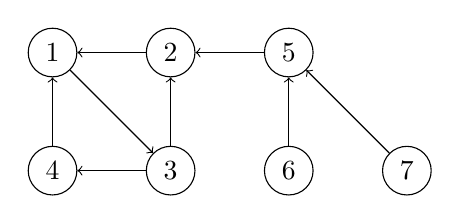
\begin{tikzpicture}[main/.style = {draw, circle},node distance={15mm}] 
        \node[main] (1) []{$1$}; 
        \node[main] (2) [right of=1] {$2$}; 
        \node[main] (3) [below of=2] {$3$}; 
        \node[main] (4) [left of=3] {$4$};
        \node[main] (5) [right of=2] {$5$};
        \node[main] (6) [below of=5] {$6$};
        \node[main] (7) [right of=6] {$7$};
        \draw[->] (2) -> (1);
        \draw[->] (4) -> (1);
        \draw[->] (3) -> (4);
        \draw[->] (1) -> (3);
        \draw[->] (3) -> (2);
        \draw[->] (5) -> (2);
        \draw[->] (6) -> (5);
        \draw[->] (7) -> (5);
        \end{tikzpicture} 
    \end{center}
Давайте теперь посмотрим, до каких вершин мы дойдем из вершины $4$: $4,1,2,3$, мы посетим только вершины текущей компоненты! Почему это так: мы не можем уйти из данной компоненты, ведь мы развернули ребра (а ребер, которые входят в эту компоненту нет, так как топсорт нам дал первую такую вершину, что она в самой первой компоненте). Но при этом в компоненте сильной связности мы можем также дойти из любой в другую даже по развернутым ребрам!
Теперь можно написать код, который сожмет граф. Каждую вершину мы пронумеруем в номер компоненты, который будет глобальной переменной $K$.

\begin{verbatim}
#include <bits/stdc++.h>
using namespace std;
int n,m;
vector<int>color;
vector<vector<int>>e; 
vector<vector<int>>e2; // обратные ребра
vector<int>path; // здесь сохраним топсорт
vector<int>comp; // здесь посчитаем номер компоненты сильной связности, в которой каждая вершина находится
int K = 0; // это количество компонент
void dfs(int x) { // этот dfs считает нам топсорт
    if(color[x]) return;
    color[x] = 1;
    for(auto& y : e[x]) {
        dfs(y);
    }
    path.push_back(x);
}
void dfs2(int x) { // этот dfs идет по обратным ребрам и считает номер компоненты
    if(color[x]) return;
    color[x] = 1;
    comp[x] = K;
    for(auto& y : e2[x]) { // идем по массиву e2, по обратным ребрам
        dfs2(y);
    }
}


int main() {
    ios::sync_with_stdio(0);
    cin.tie(0);
    cout.tie(0);
    cin >> n >> m;
    e = vector<vector<int>>(n+1);
    e2 = vector<vector<int>>(n+1);
    for(int i = 1; i <= m; i++) {
        int x,y;
        cin >> x >> y; // считываем ребра
        e[x].push_back(y);
        e2[y].push_back(x);
    }
}
\end{verbatim}
Здесь мы написали все наши основные функции. Теперь посмотрим, как будет выглядеть решение поэтапно:

\begin{center}
        \begin{tikzpicture}[main/.style = {draw, circle},node distance={80mm}] 
        \node[main] (1) []{Найти <<топсорт>>}; 
        \node[main] (2) [below of=1] {Найти компоненты сильной связности}; 
        \node[main] (3) [right of=2] {Посчитать степени вершин нового графа}; 
        \draw[->] (1) -> (2);
        \draw[->] (2) -> (3);
        \end{tikzpicture} 
    \end{center}
(Это тоже граф такой, кстати). В общем, мы уже умеем делать последний пункт, теперь отдельно рассмотрим моменты решения!
Вот так мы их потом соберем:
\begin{verbatim}
#include <bits/stdc++.h>

int main() {
    Считать граф
    Найти "топсорт"
    Найти компоненты сильной связности
    Найти степени вершин
    Найти истоки и проверить, что он один
    Достать все вершины из истока (ведь он сжатый, 
    на самом деле в оригинальном графе в одной вершине может быть несколько)
}
\end{verbatim}

Итак, начнем с поиска топсорта (это в какой-то функции, потом объединим в один код):
\begin{verbatim}
path = vector<int>(); // обнулили path
color = vector<int>(n+1); // подготовили массив цветов
for(int i = 1; i <= n; i++){
    dfs(i); 
}
reverse(path.begin(), path.end()); 
\end{verbatim}
Все, <<топсорт>> найден. Теперь конденсируем:
\begin{verbatim}
color = vector<int>(n+1); // обновляем color
K = 0; // обнуляем счетчик компонент
comp = vector<int>(n+1);
for(auto& x : path) {
    if(color[x] == 0) { // мы еще не пометили эту вершину?
        K++; // увеличиваем номер компоненты, будем помечать очередной раз
        dfs2(x);
    }
}
\end{verbatim}
После этого наш исходный граф выглядит вот так:
\begin{center}
        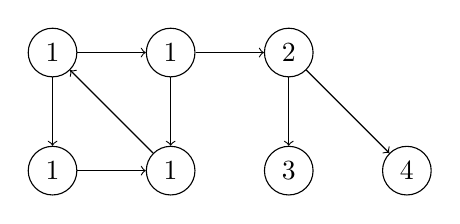
\begin{tikzpicture}[main/.style = {draw, circle},node distance={15mm}] 
        \node[main] (1) []{$1$}; 
        \node[main] (2) [right of=1] {$1$}; 
        \node[main] (3) [below of=2] {$1$}; 
        \node[main] (4) [left of=3] {$1$};
        \node[main] (5) [right of=2] {$2$};
        \node[main] (6) [below of=5] {$3$};
        \node[main] (7) [right of=6] {$4$};
        \draw[->] (1) -> (2);
        \draw[->] (1) -> (4);
        \draw[->] (4) -> (3);
        \draw[->] (3) -> (1);
        \draw[->] (2) -> (3);
        \draw[->] (2) -> (5);
        \draw[->] (5) -> (6);
        \draw[->] (5) -> (7);
        \end{tikzpicture} 
    \end{center}
Вместо номера исхдодной вершины тут номер компоненты. Мы знаем и номер оригинальной вершины $x$, а ее номер в новом графе это $comp[x]$. Главное не посчитать лишнее! Например, нас уже не интересуют ребра между вершинами одной компоненты, затем нас не интересует, из какой именно вершины компоненты мы пойдем в другую компоненту!
Заведем массив, который считает степень вершин в новом графе:
\begin{verbatim}
vector<int>in(n+1); // можно сделать размера n, количество вершин не увеличится!
for(int x = 1; x <= n; x++) {
    for(auto& y : e[x]) {
        if(comp[x] == comp[y]) continue; // это ребро в одной компоненте, зачем нам оно?
        // теперь у нас ребро в новом графе comp[x] -> comp[y]
        in[comp[y]]++; // увеличиваем степень comp[y]
    }
}
int cnt = 0; // считаем количество истоков
for(int i = 1; i <= K; i++) { // здесь уже итерируемся по номеру компоненты нового графа
    if(in[i] == 0) cnt++;
}
if(cnt > 1) {
    cout << 0 << '\n'; // больше чем один исток, ответа нет!
    return; 
}
// А иначе ответ в таких вершинах, которые лежат в компоненте, у которой степень 0!
vector<int>ans;
for(int i = 1; i <= n; i++) {
    if(in[comp[i]] == 0) ans.push_back(i);
}
cout << ans.size() << '\n';
for(auto& x : ans) {
    cout << x << ' ';
}
cout << '\n';
\end{verbatim}

Объединяем все в решение и готово:

\begin{verbatim}
#include <bits/stdc++.h>
using namespace std;
int n,m;
vector<int>color;
vector<vector<int>>e; 
vector<vector<int>>e2; // обратные ребра
vector<int>path; // здесь сохраним топсорт
vector<int>comp; // здесь посчитаем номер компоненты сильной связности, в которой каждая вершина находится
int K = 0; // это количество компонент
void dfs(int x) { // этот dfs считает нам топсорт
    if(color[x]) return;
    color[x] = 1;
    for(auto& y : e[x]) {
        dfs(y);
    }
    path.push_back(x);
}
void dfs2(int x) { // этот dfs идет по обратным ребрам и считает номер компоненты
    if(color[x]) return;
    color[x] = 1;
    comp[x] = K;
    for(auto& y : e2[x]) { // идем по массиву e2, по обратным ребрам
        dfs2(y);
    }
}

void findTopSort() {
    path = vector<int>(); // обнулили path
    color = vector<int>(n+1); // подготовили массив цветов
    for(int i = 1; i <= n; i++){
        dfs(i); 
    }
    reverse(path.begin(), path.end()); 
}
void cond() {
    color = vector<int>(n+1); // обновляем color
    K = 0; // обнуляем счетчик компонент
    comp = vector<int>(n+1);
    for(auto& x : path) {
        if(color[x] == 0) { // мы еще не пометили эту вершину?
            K++; // увеличиваем номер компоненты, будем помечать очередной раз
            dfs2(x);
        }
    }
}
void solve() {
    vector<int>in(n+1); // можно сделать размера n, количество вершин не увеличится!
    for(int x = 1; x <= n; x++) {
        for(auto& y : e[x]) {
            if(comp[x] == comp[y]) continue; // это ребро в одной компоненте, зачем нам оно?
            // теперь у нас ребро в новом графе comp[x] -> comp[y]
            in[comp[y]]++; // увеличиваем степень comp[y]
        }
    }
    int cnt = 0; // считаем количество истоков
    for(int i = 1; i <= K; i++) { // здесь уже итерируемся по номеру компоненты нового графа
        if(in[i] == 0) cnt++;
    }
    if(cnt > 1) {
        cout << 0 << '\n'; // больше чем один исток, ответа нет!
        return; 
    }
    // А иначе ответ в таких вершинах, которые лежат в компоненте, у которой степень 0!
    vector<int>ans;
    for(int i = 1; i <= n; i++) {
        if(in[comp[i]] == 0) ans.push_back(i);
    }
    cout << ans.size() << '\n';
    for(auto& x : ans) {
        cout << x << ' ';
    }
    cout << '\n';
}

int main() {
    ios::sync_with_stdio(0);
    cin.tie(0);
    cout.tie(0);
    cin >> n >> m;
    e = vector<vector<int>>(n+1);
    e2 = vector<vector<int>>(n+1);
    for(int i = 1; i <= m; i++) {
        int x,y;
        cin >> x >> y; // считываем ребра
        e[x].push_back(y);
        e2[y].push_back(x);
    }
    findTopSort();
    cond();
    solve();
}
\end{verbatim}
    
\end{document}
